\chapter{Análise Bibliográfica sobre Simulação e Ensino-Aprendizagem em Sala de Aula, por \label{chap:bibliometria:bananaMoshpit}}

\section{Planejamento do estudo}\label{S@bananaMoshpit:planejamento}

Este trabalho se refere ao estudo bibliográfico sobre o modelo de simulação multiagente de segregação racial por Thomas Schelling, daqui em diante referido como modelo de Schelling. As perguntas que nortearam este estudo foram:
\begin{itemize}
    \item Quais áreas usam a simulação de schelling? 
    \item Quais os objetivos dos estudos ao utilizarem tal modelo?
    \item Quão relevante se manteve o modelo?
\end{itemize}

\subsection{O Modelo de Schelling para segregação}
O modelo é multiagente e foi criado em 1971 pelo economista Thomas Schelling para simular a segregação residencial entre etnias. Os agentes são os indivíduos populacionas e a simulação presume que eles preferem conviver ao lado de outros de mesma etnia, portanto causando uma segregação independente de um esforço consciente \ref{hatna2012schelling}. 

O modelo é mais explicado abaixo com um exemplo de simulação realizado na implementação disponível por \citet{mccown_schellings_nodate}.
\begin{figure}
    \centering
    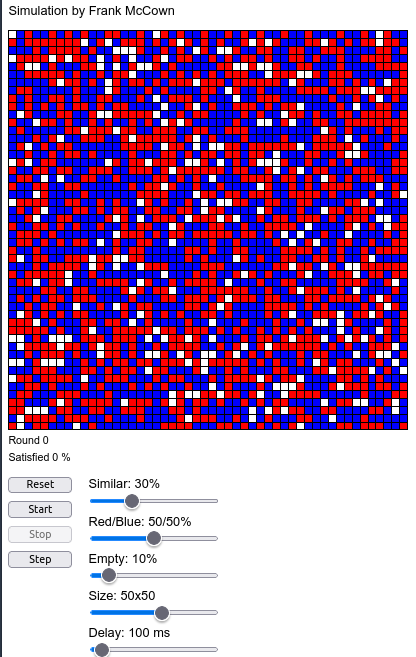
\includegraphics[width=0.6\textwidth]{exploratory-data-analysis/bananaMoshpit/PesqBibliogr/SimulacaoMultiagente/schelling-FM-initial.png}
    \caption{Estado inicial de simulação do modelo de schelling-- iteração 0. Fonte: \citet{mccown_schellings_nodate}}
    \label{STL@bananaMoshpit-schelling-init}
\end{figure}

Os quadrados brancos e azuis são indivíduos-- cada um de sua respectiva 'classe' (econômica, cultural, étnica, etc.), enquanto que os brancos são 'espaços vazios'. Inicialmente, nota-se que muitos indivíduos são vizinhos diretos de agentes de outra classe. Explicando os parâmetros de simulação-- a configuração 'similar' define a linha de satisfação do agente; no caso, um agente está satisfeito se 30/100 de seus vizinhos compartilharem de sua classe. A configuração 'Red/Blue' define a percentagem populacional denotada pelas duas classes; no caso, o total de agentes é dividido igualmente entre as duas classes. A 'Empty' define a quantidade de espaços em brancos; no caso, 10/100 da malha de simulação. 'Size' define o tamanho de malha de simulação; no caso, 50x50 blocos. Por fim, 'Delay' define o tempo de espera entre cada iteração; no caso, 100ms. Segue  resultado dessa simulação abaixo.

\begin{figure}
    \centering
    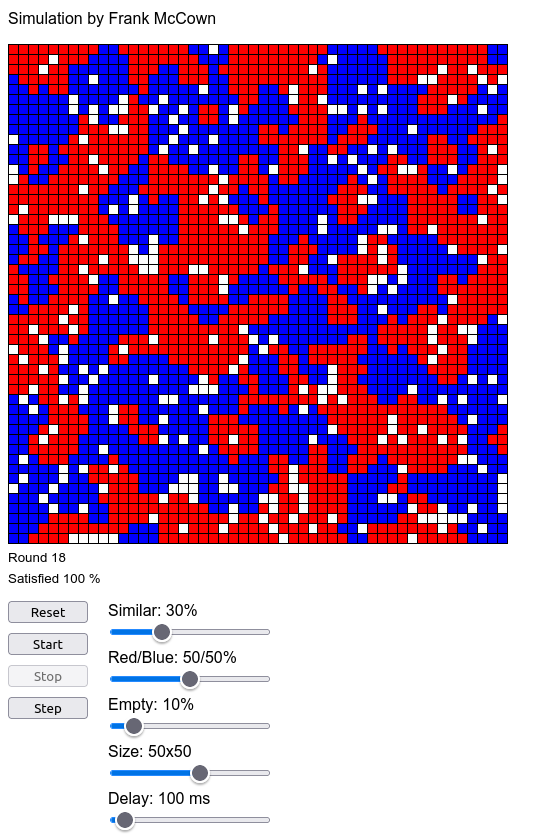
\includegraphics[width=0.6\textwidth]{exploratory-data-analysis/bananaMoshpit/PesqBibliogr/SimulacaoMultiagente/schelling-FM-final.png}
    \caption{Estado final de simulação do modelo de schelling-- iteração 18. Fonte: \citet{mccown_schellings_nodate}}
    \label{STL@bananaMoshpit-schelling-final}
\end{figure}

Notoriamente, os agentes se reorganizaram na malha de simulação e segregaram por classe-- note que o estado final da simulação possui mais indivíduos completamente rodeados por vizinhos de mesma classe. Esta é a finalidade do modelo de schelling: simular a segregação de agentes por classe. 


\subsection{Uso do Bibliometrix e Biblioshiny}

Foram usadas a ferramenta e o \textit{workflow} proposto pelos autores do pacote Bibliometrix \cite{aria_bibliometrix_2017}.

\subsection{Limitações} O exercício relatado foi feito em 4 dias, envolvendo entre 15 e 20 horas de trabalho.

\section{Coleta de dados\label{S@bananaMoshpit:coleta}}

A coleta de dados feita usando o banco de dados SCOPUS no dia 07 de agosto de 2022, acessado por meio de seu portal oficial e gratuito de pesquisa acadêmica \ref{SCOPUSsearch}, sem especificação de coleções ou outros filtros.

\subsection{Query de Busca}
Foi usada a \query\  de busca ilustrada nas linhas 1 a 9 da listagem \ref{bananaMoshpitQuery-20221207}.

\lstinputlisting[numbers=left,basicstyle=\normalsize\ttfamily,caption={\query\  de busca relacionado à simulação multiagente de segregação geográfica por componente étnico, especialmente pesquisas referentes ao modelo de \citet{mccown_schellings_nodate}} ,label=bananaMoshpitQuery-20221207]
{exploratory-data-analysis/bananaMoshpit/PesqBibliogr/SimulacaoMultiagente/SCOPUS-20221207/query.txt}

\subsubsection{Explicação para os termos de busca usados}

A busca final consistiu de sete cláusulas disjuntivas e três conjuntivas, onde cada termo poderia comparecer no título da publicação, em seu resumo ou em suas palavras-chave.

Os termos \texttt{mesa}, \texttt{python*}, \texttt{agent}, \texttt{simulat*}, e \texttt{sym} (linha 9 da query) garantem que os resultados se refiram à modelos computacionais, especificamente à interface 'mesa', a lingaguem de programação 'python', a simulações 'multi-agent' e a 'simulações' ('simulation' ou sua abreviação 'sym').

Já os termos \texttt{schelling*}, \texttt{segreg*}, \texttt{rac*} e \texttt{ethni*}(linhas 2 e 4 da query) foram usados na primeira cláusula da \query\  para recuperar artigos referentes à modelos relacionados aos termos 'segregação racial, étinca ou geográfica' ou ao nome do modelo de estudo base deste artigo:'schelling'. Por fim, os termos \texttt{schelling*} e \texttt{residen*} (linha 6) incluem também a possibilidade de artigos relacionados a 'segregação residencial e o modelo de schelling'-- porém não são permitidos resultados mencionando apenas 'segregação' e 'residencial', porque estes permitem resultados quantitativos e além do escopo do modelo de schelling.

\subsection{Registros recuperados}

O resultado da busca obteve 500 registros. Exportou-se uma listagem dos mesmos, utilizando \textit{Export->RIS Export} após a busca da \textit{query}, com todas as opções marcadas como ilustrado abaixo.

\begin{figure}
    \centering
    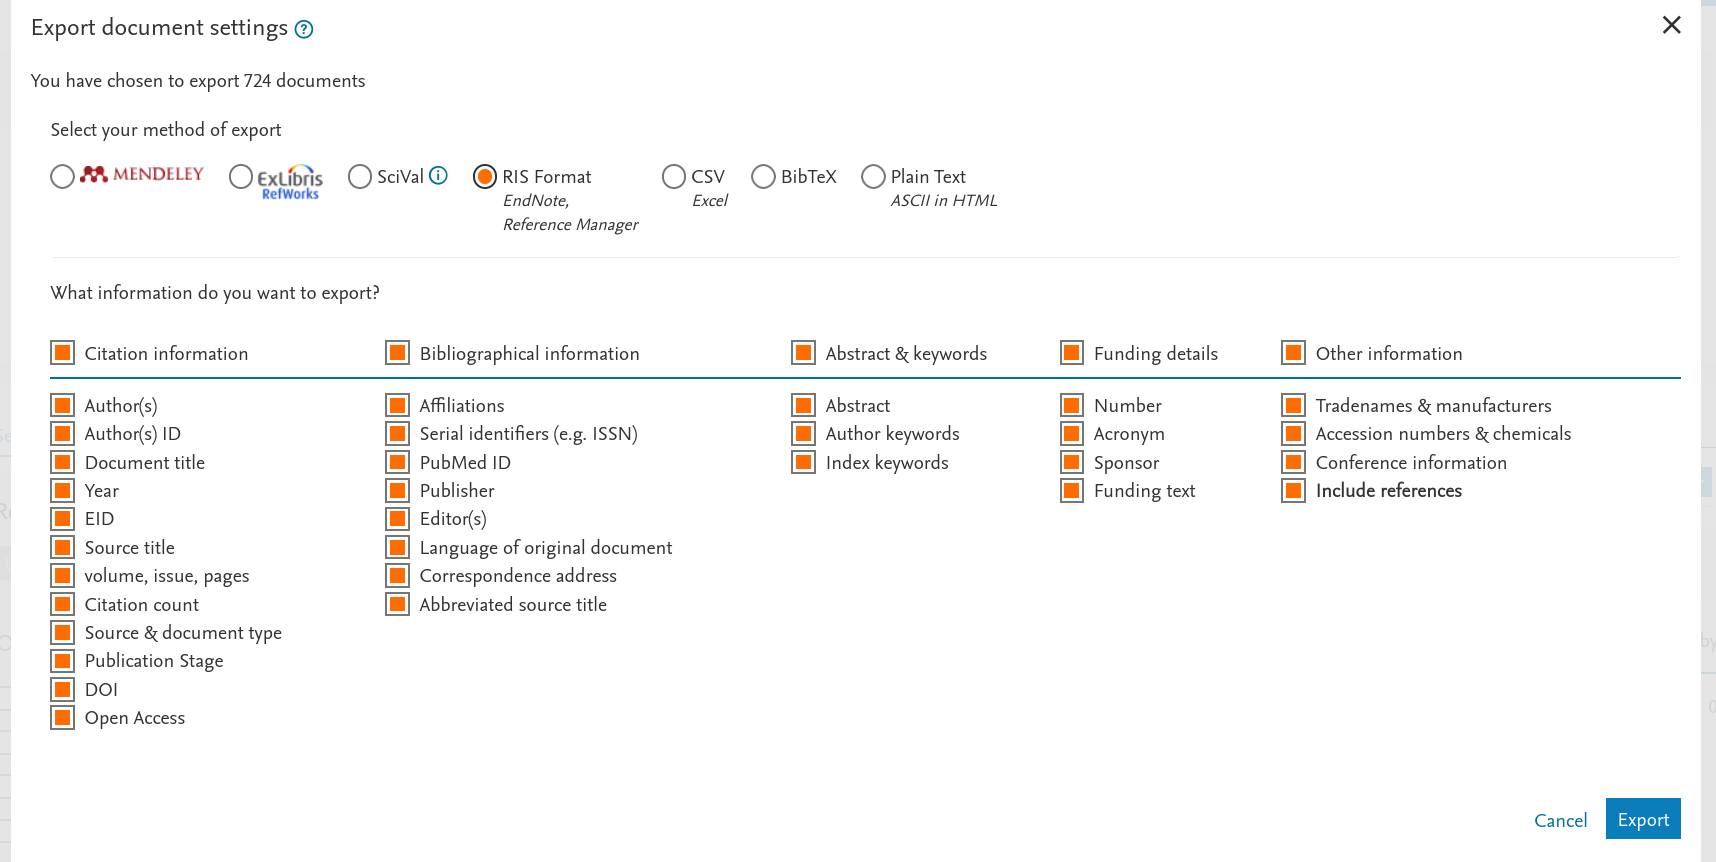
\includegraphics[width=1.2\textwidth]{exploratory-data-analysis/bananaMoshpit/PesqBibliogr/SimulacaoMultiagente/SCOPUS-20221207/export-settings.png}
    \caption{Exportando bibliografia da base SCOPUS}
    \label{STL@bananaMoshpit-SCOPUS-extract}
\end{figure}

Dessa forma, a listagem das bibliografias extraida está armazenada em  \url{https://github.com/jhcf/Comput-Experim-20212-Overleaf2/exploratory-data-analysis/bananaMoshpit/PesqBibliogr/SimulacaoMultiagente/SCOPUS-20221207/500records.txt} .

\section{Análise dos dados\label{S@bananaMoshpit:analise}}
A listagem obtida em \ref{S@bananaMoshpit:coleta} resultou em um dataset de 500 registros. Utilizando a função biblioAnalysis() da bibliometrix, obteve-se a seguinte análise de dados:

MAIN INFORMATION ABOUT DATA

 Timespan                              1975 : 2023 
 Sources (Journals, Books, etc)        381 
 Documents                             500 
 Annual Growth Rate %                  0 
 Document Average Age                  10.1 
 Average citations per doc             24.14 
 Average citations per year per doc    2.036 
 References                            23187 


 \section{Visualização dos dados\label{S@bananaMoshpit:visualizacao}}
 Extraídos com a interface biblioshiny para bibliometrix, conseguiram-se os dados:



 
 \section{ Interpretação dos dados\label{S@bananaMoshpit:interpretacao}}
